\documentclass[a4paper,11pt]{article}

\usepackage[english]{babel}
\usepackage[utf8x]{inputenc}
\usepackage{amsmath,amssymb,amsthm}
\usepackage{graphicx}
\usepackage{lineno}
%include the code below (between the comments) to get lineno to work better
\newcommand*\patchAmsMathEnvironmentForLineno[1]{%
  \expandafter\let\csname old#1\expandafter\endcsname\csname #1\endcsname
  \expandafter\let\csname oldend#1\expandafter\endcsname\csname end#1\endcsname
  \renewenvironment{#1}%
     {\linenomath\csname old#1\endcsname}%
     {\csname oldend#1\endcsname\endlinenomath}}% 
\newcommand*\patchBothAmsMathEnvironmentsForLineno[1]{%
  \patchAmsMathEnvironmentForLineno{#1}%
  \patchAmsMathEnvironmentForLineno{#1*}}%
\AtBeginDocument{%
\patchBothAmsMathEnvironmentsForLineno{equation}%
\patchBothAmsMathEnvironmentsForLineno{align}%
\patchBothAmsMathEnvironmentsForLineno{flalign}%
\patchBothAmsMathEnvironmentsForLineno{alignat}%
\patchBothAmsMathEnvironmentsForLineno{gather}%
\patchBothAmsMathEnvironmentsForLineno{multline}%
}
%the code is above
\linenumbers

\newtheorem{prop}{Proposition}

% Don't change the settings above. For example, the line numbers make for easy counting of the length of a piece of work.
% Don't change margins, fonts (including size) or make any other alterations which would either expand or contract the length of the resulting file. 
% You can add packages if you need but these should not impact on the length of the document, the markers have discretion to determine if such additions are appropriate. You should not need to add any packages for the first assignment.

 

\title{HCoV Skills Assignment 1}
\author{Li Yueheng, s2306076}

\begin{document}
\maketitle

% What follows is poor. Make it good - see the Assignment 1 marking guide on Learn.


\section{Communication exercise} % lines formatted like this should be section headings

\begin{figure}[h]\label{fig_example_figure}
    \centering
    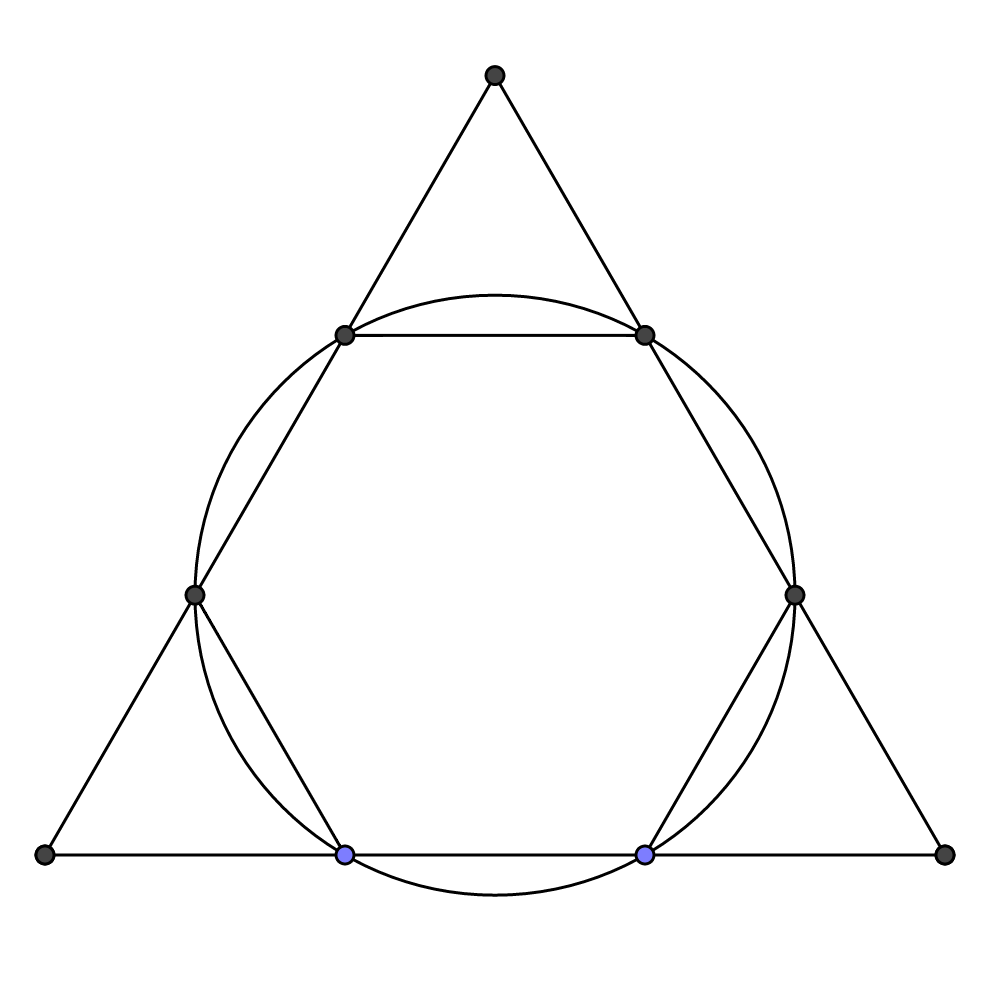
\includegraphics[width=0.4\textwidth]{d7.png}
    \caption{Example Figure}
\end{figure}

Figure \ref{fig_example_figure} consists of a hexagon cut from the outside by a circle. Two of the hexagon's neighboring  vertices are colored blue. Three non-neighboring edges of the hexagon, including the one joining the blue vertices, are extended to form an equilateral triangle. All vertices but the two blue ones are colored black.




\section{Holomorphic functions}

\begin{prop}\label{prop:fCtoRconst} % Leave this proposition as it is.
Suppose the function \( f \) is holomorphic on \( \mathbb{C} \) and takes only real values. It follows that \( f \) must be constant.
\end{prop}

\begin{proof}
Since $f$ is holomorphic on the complex plane $\mathbb{C}$, it should satisfy the Cauchy-Riemann equations anywhere on $\mathbb{C}$. Since $f$ takes only real values, from the Cauchy-Riemann equations we have
\begin{align*}
	&\partial_x f=\partial_y 0=0 \\
	&\partial_y f=-\partial_x 0 =0
\end{align*}
Therefore $f$ is continuously differentiable on $\mathbb{C}$. By the Fundamental theorem of Calculus, $f$ is a constant function on any line parallel to the x-axis or the y-axis. It follows that $f$ is a constant function on $\mathbb{C}$.
\end{proof}


\section{Microwriting}

Plagiarism is the act of copying others' work without appropriate acknowledgement or one's own previously assessed, either intentionally or unintentionally.\cite{1}

Collusion is a particular type of plagiarism, where students work in unauthorized collaboration to complete an assessed work.\cite{1}

Suspected academic misconduct, including plagiarism and collusion will lead to an investigation conducted by the university's officials, who will determine appropriate penalties for confirmed academic misconduct. These penalties might include grade penalties, disciplinary actions and even expulsion from the university.\cite{2,3}

\begin{thebibliography}{99}

	\bibitem{1} https://teaching.maths.ed.ac.uk/main/undergraduate/studies/assessment/academic-misconduct
	
	\bibitem{2}https://www.scanmyessay.com/plagiarism/consequences-of-plagiarism.php
	
	\bibitem{3}https://www.scribbr.co.uk/preventing-plagiarism/consequences-of-plagiarism/
\end{thebibliography}

\end{document}